\chapter{Implementation}

\section{Configuration Management Guide}
In this section, we define a guide helping us programming and defining our structures in a homogene in order to easily read each other and to help the integration of our separate codes. This, since we programmed on the same prototype seperately. This document help us have homogenized codes on python.
\paragraph{}


\paragraph{Structure code :} For every languages used, we will prefer the definition of code in two parts:
\begin{itemize}
\item First part: definition of functions and procedures or methods;
\item Second part: Main function.
\end{itemize}


This process reduces the recall of certain calculations and allow to have a better visibility of code. It is necessary follow the order of definition for compilation.


\paragraph{Comments :} Each different parts should have a brief description before it is edited.
functions and procedures have a functional description;
tvariables are commented after their definition.


\paragraph{Definition of variables :} 
\begin{itemize}
\item Variables are defined at the beginning of each entity (functions, procedures, classes, hands etc ...) except possibly in object-oriented programming;
\item The name of a variable, whether local or global, is the simplest possible and defined in lowercase;


\item we will take care to separate input variables from those output for better visibility.
\end{itemize}

\paragraph{Definition of functions, procedures or methods :} 
\begin{itemize}
\item As with object-oriented programming (JAVA) we will take for a function, at least two significant words with the first word in lowercase letters and the first letter of the second word capitalized. It provides for example in case of two words "calculateMatrix" and three words "calculateScatterMatrix".
\end{itemize}


\paragraph{Definition of classes :} 
\begin{itemize}
\item Classes are defined in capital letters(first letter), they are the superior entities after the Object class.
\end{itemize}

\paragraph{Definition of Main :} 
\begin{itemize}
\item Before each function call comment out by a significant title.
\end{itemize} 

\paragraph{Identation :} 
\begin{itemize}
\item Carefully idente your code.
\end{itemize} 

\section{Implementation results}
As said lately,for the implementation of eigenfaces method we used AT\&T database  composed of 400 images. The database consists of 40 subjects and each subject has 10 images.

We illustrate hereinater some images of the database :
\begin{figure}[bth]%[!ht]
\begin{center}
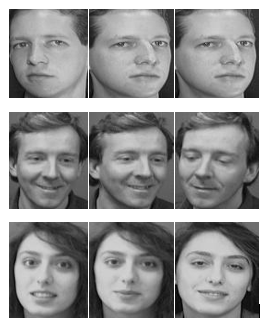
\includegraphics[scale=0.75,height=70mm,width=70mm]{capture_img}%[height=15cm,width=17cm]
\caption{\textbf{images of database }}%
%\url {http://www.google.fr/}
%\label{learningPhaseGM}
\end {center}
\end{figure}
\\All images of database are loading from directory by the function \textbf{read\_img.py}(annexes).
After that,the average of all images of the database will be calculated by the functiun \textbf{computeMeanImage\_.py} and centered by \textbf{computeCenteredImage\_.py}.
\\The average image is a vector and for saved it we needed to  convert it into a matrix(annexes).
\clearpage
The illustration of average image is :

\begin{figure}[bth]%[!ht]
\begin{center}
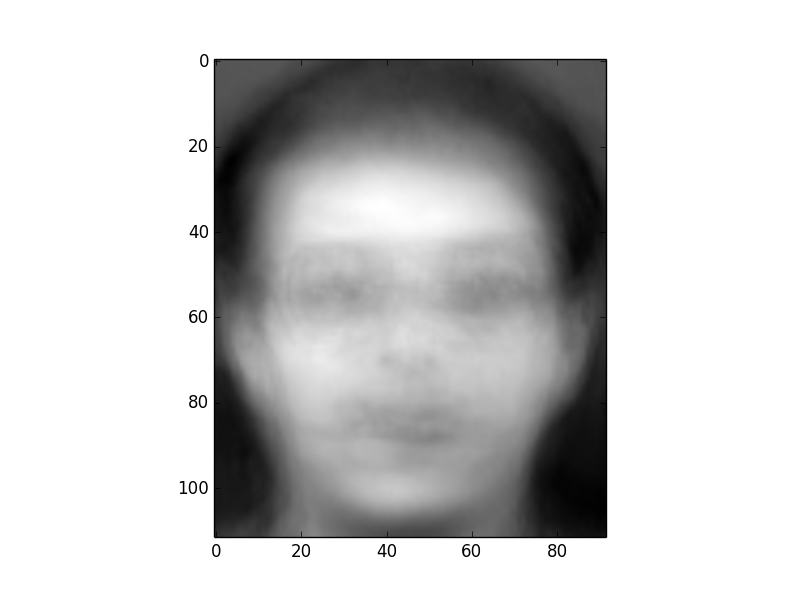
\includegraphics[scale=0.75]{figure_1}%[height=15cm,width=17cm]
\caption{\textbf{Average image }}%
%\url {http://www.google.fr/}
%\label{learningPhaseGM}
\end {center}
\end{figure}
The average image is fluzzy because many images are used.
\clearpage
\section{Integration into Oriented Programming Language}
In order to create Objects from our prototype we designed the main classes presented as following :

\begin{figure}[bth]%[!ht]
\begin{center}
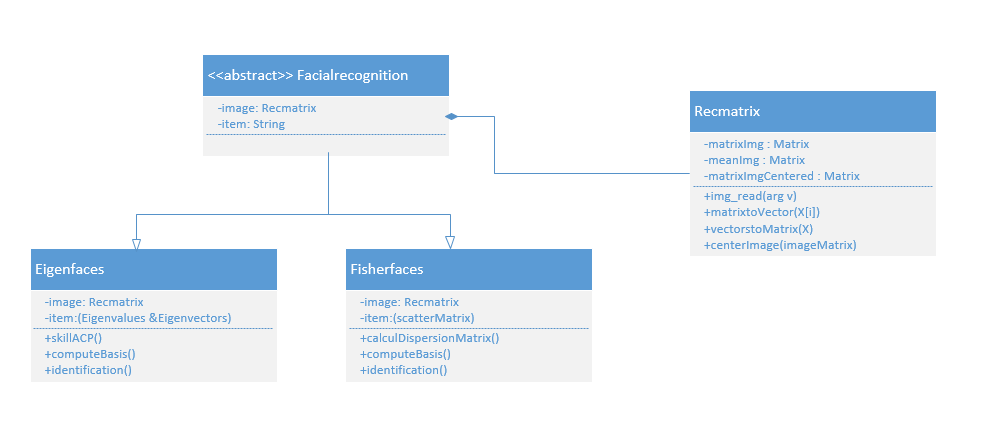
\includegraphics[scale=0.85,height=10cm,width=14cm]{diag_uml}%[height=15cm,width=17cm]
\caption{\textbf{UML Flowchart }}%
%\url {http://www.google.fr/}
%\label{learningPhaseGM}
\end {center}
\end{figure}


\section{Prospects}
Facial recognition develop tools very useful for people such as our first goals which were to improve parental control and to develop serious in order to help childrens with handicap. But so far, still there are some applications like high security, and ... All those applications require less human efforts, and then the use of this method are factor of unemployement and reduce responsibility from parents.
On this project, we would have expected to have much more time to implement the methods in other way and to optimize much more the programs.

\clearpage
\section{Difficulties faced and summary}
%\section{Difficultés rencontrés et Bilan}
\subsection{Difficulties faced}

When the project began, we set several objectives. To achieve them, we have established a  schedule for work organized. But throughout the project, we have encountered some difficulties: technical difficulties and organizational difficulties.
\paragraph{} 
The main difficulties are :
\begin{itemize}
\item implementation difficulties : because for programming methods, we had to define a unique way to structure the program for consistency in all codes. We have thus established a reference document to have uniform codes.
\item understanding difficulties :everyone had understood in a different way from others  the concept of the methods(eigenfaces and fisherfaces) for the implementation of our algorithm. 
\item Programming difficulties :we have different levels in programming. But that does not prevent us to program
\item Using tools  difficulties : everyone had to program a part of the code, so we needed a way for share and  synchronize our codes. the tool was new and we took time to control this,
\item management difficulties : as we have already said, we set goals and we had established a schedule for work in an organized way, but many secondary, unanticipated and unforeseeable tasks appeared.
\end{itemize}

However we faced all these difficulties, which allowed us to learn more about the two main domain of our project: images processing and programming language .
Finally, these difficulties may be helpful for future work. These can be apprehended in another project


\subsection{Summary}

This project allowed us to gain maturity in the work and help us  to understand the importance of schedule, organization, and discipline necessary to achieve a project. In addition, it also gave us the satisfaction of completing the project in a group. Each member benefits from the skills of other members. That share of skills and the adding skills we have gained make us think it is such a very positive experience to our training and future carreer. Because this experience has allowed us to figure out the complexity to manage a project, but also the difficulty of understanding and the importance of communication in a group.


